\documentclass[12pt]{article}
\usepackage{amsmath}
\usepackage{array}
\usepackage[thinc]{esdiff}
% \usepackage{gensymb}
\usepackage{geometry}
\usepackage{graphicx}
\usepackage{pgfplots}
\usepackage{siunitx}
\usepackage{wrapfig}

\title{Homework \#3, 4B}
\author{Donald Aingworth IV}
\date{February 5, 2025}

\pgfplotsset{width=8cm,compat=1.9}
\usepgfplotslibrary{external}
% \tikzexternalize

\begin{document}

\DeclareSIUnit{\mile}{mi}
\DeclareSIUnit{\gal}{gal}
\DeclareSIUnit{\foot}{ft}
\DeclareSIUnit{\hour}{h}
\DeclareSIUnit{\rad}{rad}
\DeclareSIUnit{\unit}{u}
\DeclareSIUnit{\dyne}{dyn}

\maketitle

\section{Problem 33}
\begin{wrapfigure}{r}{0.5\textwidth}
    \vspace{-30pt}
    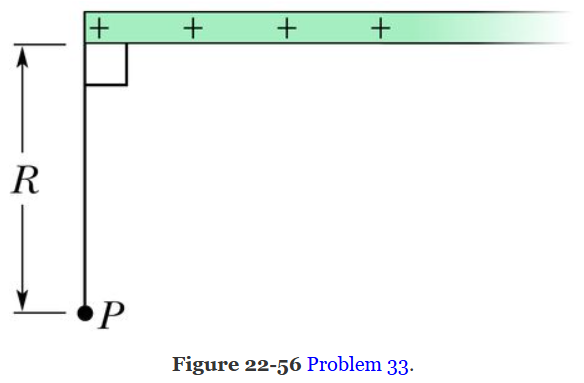
\includegraphics[width=0.5\textwidth]{picture_1.png} 
    % \label{fig:wrapfig}
\end{wrapfigure}
Fig. 22-56, a "semi-infinite" nonconducting rod (that is, infinite in one direction only) has uniform linear charge density $\lambda$. Show that the cetric field $E_p$ at point $P$ makes an angle of 45\unit{\degree} with the rod and that this result is independent of the distance $R$. (Hint: separately find the component of $E_p$ parallel to the rod and the component perpendicular to the rod.)

\section{Problem 50}
At some instant the velocity components of an electron moving between two charged parallel plates are $U_x = 1.5 \times 10^5 \unit{\meter/\second}$ and $v_y = 3.0 \times 10^3 \unit{\meter/\second}$. Suppose the electric field between the plates is uniform and given by $\vec{E} = (120 \unit{\newton/\coulomb})\hat{j}$. In unit-vector notation, what are (a) the electron's acceleration in that field and (b) the electron's velocity when its x coordinate has changed by 2.0 cm?

\section{Problem 55}
A uniform electric field exists in a region between two oppositely charged plates. An electron is released from rest at the surface of the negatively charged plate and strikes the surface of the opposite plate, 2.0 cm away, in a time $1.5 \times 10^{-8} \unit{\second}$. (a) What is the speed of the electron as it strikes the second plate? (b) What is the magnitude of the electric field $\vec{E}$?

\section{Problem 59}
How much work is required to turn an electric dipole 180\unit{\degree} in a uniform electric field of magnitude E = 46.0 N/C if the dipole moment has a magnitude of $p = 3.02 \times 10^{-25} \unit{\coulomb\cdot\meter}$ and the initial angle is 64\unit{\degree}?

\section{Problem 60}
\begin{wrapfigure}{r}{0.25\textwidth}
    \vspace{-30pt}
    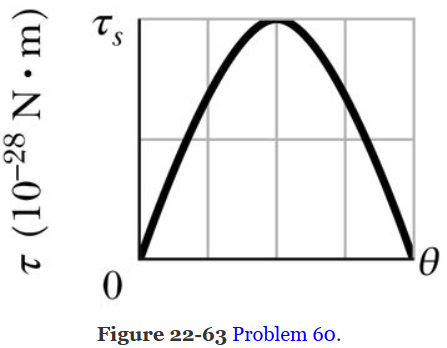
\includegraphics[width=0.25\textwidth]{picture_5.png} 
    % \label{fig:wrapfig}
\end{wrapfigure}
A certain electric dipole is placed in a uniform electric field E of magnitude 40 N/C. Figure 22-63 gives the magnitude $\tau$ of the torque on the dipole versus the angle $\theta$ between field E and the dipole moment p. The vertical axis scale is set by $\tau_s = 100 \times 10-28 \unit{\newton\cdot\meter}$. What is the magnitude of p?

\section{Problem 76}
\begin{wrapfigure}{r}{0.15\textwidth}
    \vspace{-30pt}
    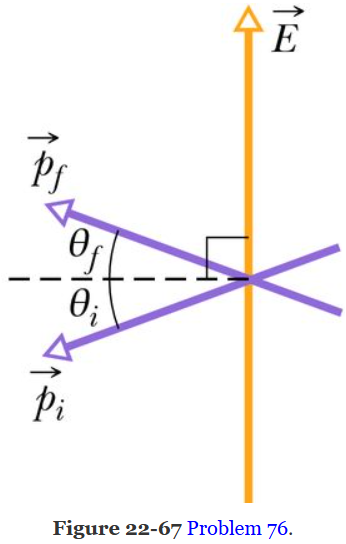
\includegraphics[width=0.15\textwidth]{picture_6.png} 
    % \label{fig:wrapfig}
\end{wrapfigure}
In Fig. 22-67, an electric dipole swings from an initial orientation $i (\theta_i = 20.0\unit{\degree})$ to a final orientation $f (\theta_f= 20.0\unit{\degree})$ in a uniform external electric field E. The electric dipole moment is $1.60 \times 10^{-37} \unit{\coulomb\cdot\meter}$; the field magnitude is $3.00 \times 10^6 \unit{\newton/\coulomb}$. What is the change in the dipole's potential energy?

\end{document}